\section*{Câu 4.3.1 --- Mô hình phân lớp tuyến tính \& hàm chi phí trên tập sai}

Cho tập huấn luyện gồm 4 mẫu $(x_k,t_k)$ với $x_k=(x_{k1},x_{k2})\in\mathbb{R}^2$, $t_k\in\{-1,+1\}$:
\[
\begin{aligned}
&x_1=(1,1),\ t_1=+1; &&x_2=(2,1),\ t_2=+1;\\
&x_3=(1,2),\ t_3=-1; &&x_4=(2,2),\ t_4=-1.
\end{aligned}
\]
Mô hình dự đoán $\hat y=\mathrm{sign}(w^\top x+b)$ với
\[
\mathrm{sign}(z)=\begin{cases}+1,& z\ge 0,\\ -1,& z<0.\end{cases}
\]
Gọi $Y$ là tập các mẫu bị phân lớp sai. Hàm chi phí
\[
J(w,b)=\sum_{k:\, x_k\in Y}(-t_k)\bigl(w^\top x_k+b\bigr).
\]
Khởi tạo $w^{(0)}=(1,1)^\top$, $b^{(0)}=0$.

\paragraph{(a) Các mẫu bị phân sai}
Với $w=(1,1)$, $b=0$ ta có $w^\top x+b=x_1+x_2$.
\begin{align*}
\text{Mẫu 1: }&1+1=2\ge 0 \Rightarrow \hat y_1=+1=t_1 &&\text{(đúng)}\\
\text{Mẫu 2: }&2+1=3\ge 0 \Rightarrow \hat y_2=+1=t_2 &&\text{(đúng)}\\
\text{Mẫu 3: }&1+2=3\ge 0 \Rightarrow \hat y_3=+1\neq t_3=-1 &&\text{(sai)}\\
\text{Mẫu 4: }&2+2=4\ge 0 \Rightarrow \hat y_4=+1\neq t_4=-1 &&\text{(sai)}
\end{align*}
Vậy tập phân sai gồm \textbf{mẫu 3 và mẫu 4}; kí hiệu $\mathcal Y=\{3,4\}$ (chỉ số mẫu).

\paragraph{(b) Đạo hàm của $J$}
Viết $J(w,b)=\sum_{k\in\mathcal Y}(-t_k)(w^\top x_k+b)$. Do mỗi số hạng tuyến tính theo $w$ và $b$,
\[
\frac{\partial J}{\partial w}=\sum_{k\in\mathcal Y}(-t_k)\,x_k,\qquad
\frac{\partial J}{\partial b}=\sum_{k\in\mathcal Y}(-t_k).
\]
Tại các mẫu sai có $t_3=t_4=-1$, nên $-t_3=-t_4=1$:
\[
\frac{\partial J}{\partial w}=x_3+x_4=(1,2)+(2,2)=(3,4),\qquad
\frac{\partial J}{\partial b}=1+1=2.
\]

\paragraph{(c) Một bước thuật toán Perceptron (Rosenblatt)}
Với tốc độ học $\rho=1$, khi xét \textbf{mẫu sai đầu tiên} trong thứ tự $1,2,3,4$ là mẫu 3 với $x_3=(1,2)$, $t_3=-1$, ta cập nhật
\[
w^{(1)}=w^{(0)}+\rho\,t_3\,x_3=(1,1)+(-1)(1,2)=(0,-1),\qquad
b^{(1)}=b^{(0)}+\rho\,t_3=0+(-1)=-1.
\]
Đường ranh giới mới: $w^{(1)\top}x+b^{(1)}=-x_2-1=0$, tức $x_2=-1$.

\begin{figure}[h]
   \centering
   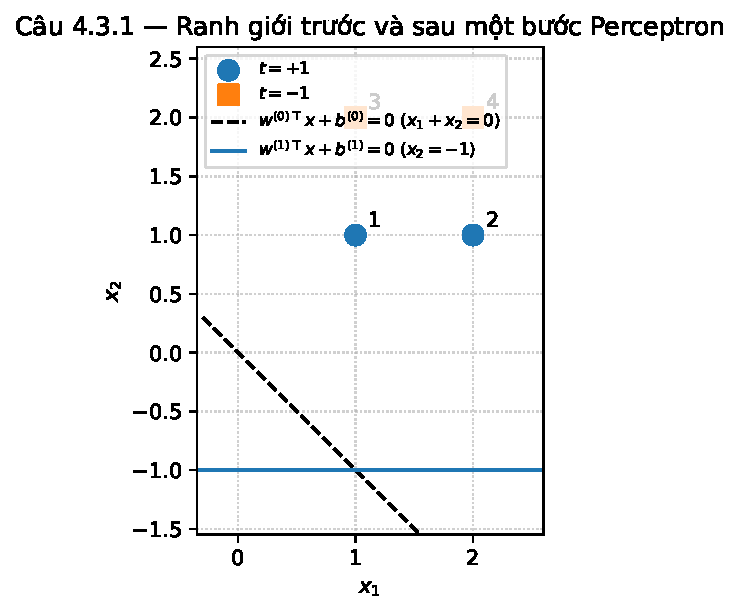
\includegraphics[width=0.68\linewidth]{figures/cau4_3_boundary.pdf}
   \caption{Các mẫu (tròn: $t=+1$, vuông: $t=-1$) và đường quyết định ban đầu $x_1+x_2=0$, sau một bước Perceptron $x_2=-1$.}
\end{figure}
